\documentclass[main.tex]{subfiles}

\newcommand{\LeptonInjector}{\texttt{LeptonInjector}}
\newcommand{\LeptonWeighter}{\texttt{LeptonWeighter}}
\newcommand{\NuGen}{\texttt{NuGen}}
\newcommand{\ANIS}{\texttt{ANIS}}
\newcommand{\Python}{\texttt{Python }}
\newcommand{\MCEq}{\texttt{MCE{\scriptsize Q}}}
\newcommand{\MMC}{\texttt{MMC}}
\newcommand{\PROPOSAL}{\texttt{PROPOSAL}}
\newcommand{\CORSIKA}{\texttt{CORSIKA}}
\newcommand{\MUONGUN}{\texttt{MuonGun}}
\newcommand{\PHOTOSPLINE}{\texttt{Photospline}}
\newcommand{\boost}{\texttt{Boost}}
\newcommand{\hdf}{\texttt{HDF5}}
\newcommand{\boostpython}{\texttt{boost-python}}
\newcommand{\nusim}{\texttt{NUSIM}}



\newcommand\pythonstyle{\lstset{
    language=Python,
    basicstyle=\footnotesize,
    otherkeywords={self},             % Add keywords here
    keywordstyle=\color{deepblue},
    emph={MyClass,__init__},          % Custom highlighting
    emphstyle=\color{deepred},    % Custom highlighting style
    stringstyle=\color{deepgreen},
    %frame=tb,                         % Any extra options here
    showstringspaces=false            % 
}}

% Python for external files
\newcommand{\pythonexternal}[2][]{{
\pythonstyle
\lstinputlisting[#1]{#2}}}


% Python for inline
\newcommand\pythoninline[1]{{\pythonstyle\lstinline!#1!}}



% Cowan_2011
\begin{document}

\section{The String 37 Offset}\label{app:pork}

Rumor has it a case of pork chops was air-dropped about 500 meters from the old south pole station long ago in the 1970s. 
Perhaps its parachute never opened, or perhaps it simply fell silently into the dense and billowing snow. 
All we can surmise is that despite their determined efforts, the polar residents were unable to find their lost and frozen dinner, and some things that should not have been forgotten were lost. 
And for three and a half decades the crate passed out of all knowledge. 

Until, when chance came, it bubbled up into relevance once more.
In the 2008-2009 South Pole season, drilling crews repeatedly hit obstacles as the hot water drill melted its way along a three kilometer deep journey. 
The solution to these obstacles would draw inspiration from film; taking a pump, an air compressor, and some spare jet fuel, driller Dennis Duling of IceCube fashioned an improvised flame-thrower to burn refuse out of the way of the IceCube hot water drill. 
But, on one particular pass the drill was pulled back to the surface with what appeared to be part of a frozen pork chop adhered to the side of the drill. 
Looking into the partially melted column, the team saw what can only be described as \textit{horrifying} and \textit{shown in Figure~\ref{fig:pork}}. 
Unsure of what they had unearthed, the drill crews elected to move the drill site several meters away into untainted ice. 
Whatever else rested within that hole will stay there, in the glacier, frozen for eons.


In general, these obstacles are what have lead to IceCube's non-perfect grid. The top-right notch missing in Figure~\ref{fig:icecube_figs} (right) is due to its proximity to the ``old pole'' station. 
Drillers found too much debris in that area which would interfere with drilling, and so the strings that would've been installed there were instead moved into DeepCore.
This is why strings 79 and 80 were placed at an odd, internal location. 
Although now, much of this story may be apocryphal, the story of the pork hole is undeniably true as evidenced by the picture of the pork itself. 
%There is also another image in the internal IceCube gallery: where there is an image of Eric Blaufass celebrating the finishing of hole 37, dubbed the ``pork hole'' in the title of the image.

\begin{figure}
    \centering
    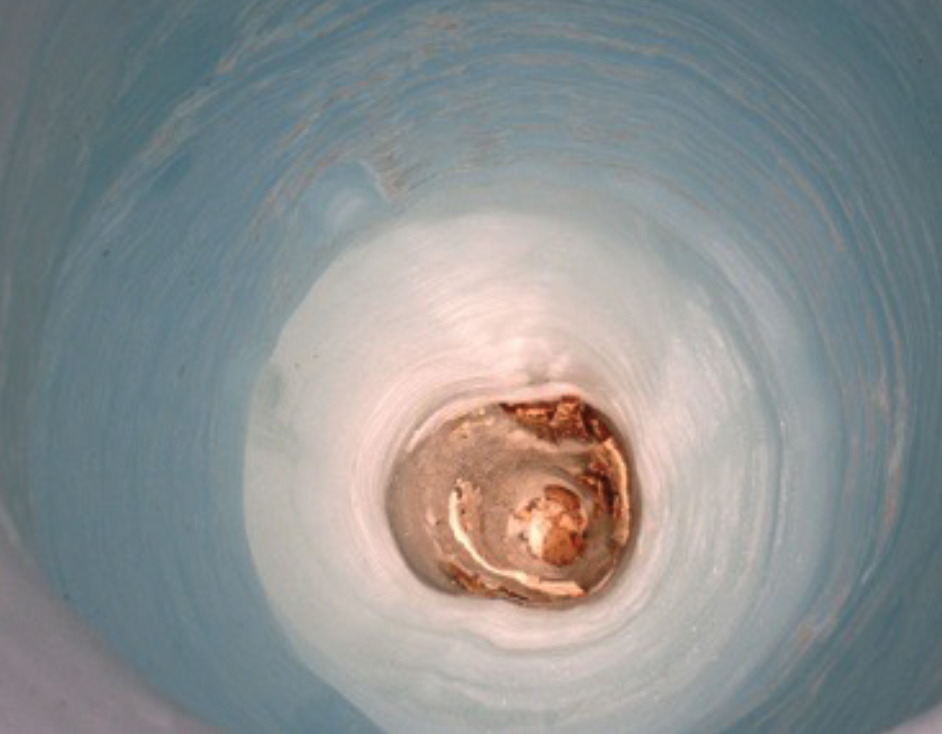
\includegraphics[width=0.6\linewidth]{figures/porkchops.png}
    \caption{Drilling of the hole for string 37 was delayed when the drill operators noticed pork chops were floating to the surface of the hole.}\label{fig:pork}
\end{figure}

%\section{Example D-Egg FAT Summary}\label{append:degg_fat}
%\includepdf[pages=-]{./degg_result.pdf}

\end{document}